\scanpage{17}
\mspage{8}
$\mathcal Z_i\subset\mathcal X_i$ et $Z\simeq\mathcal Z_1$, $Z\simeq\mathcal Z_2$).

\uline{NB} On fera attention que contrairement à ce qui se passe dans $\deleted{\unsure{\operatorname{Cat}}}\inserted{\operatorname{Esp}}_{\mathcal M_*}$) un sous-objet d'un objet $\mathcal X$ de $\underrightarrow{\operatorname{Esp}}_{\mathcal M_*}$ i.e. d'un esp. ind-modéré, ne correspond pas néc. à une partie $\mathrm{loc}^{\mathrm t}$ modérée\ldots

\figure{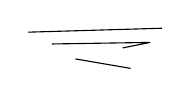
\begin{tikzpicture}\draw (0,0)--(1.7,.05);\draw (.3,-.15)--(1.55,-.13)--(1.2,-.2);\draw (.6,-.34)--(1.3,-.46);\end{tikzpicture}}
\figure{\begin{tikzpicture}\node[draw,ellipse] {$\overline{\mathrm V}$};\end{tikzpicture}}
\uline{\unsure{Relations|Relation} aux topologies} Supposons $R$ muni d'une topologie, donc les $R^I$ et les ``modèles'' modérés aussi. On voudrait que les applications modérées soient continues --- c'est OK si les parties modérées sont compactes (donc fermées, si $R$ séparé), c'est le cas. \deleted{Si le foncteur $X\mathrel{\mapstochar\relbar}$} \inserted{Supposons donc}
\figure{\begin{tikzpicture}\node[draw,ellipse] {$M9$};\end{tikzpicture}}
\[
 \left\{\begin{array}{l}R\text{ séparé}\\
 \text{les parties modérées de }R^n\text{ sont compactes}
 \end{array}\right.
\]
Alors le foncteur $X\mathbin{-}|X|$ se factorise par la cat. des espaces topologiques
\[
 \operatorname{Esp}_{\mathcal M_*}\longrightarrow(\deleted{\unsure{R|E}}\inserted{\mathrm E}\mathrm{sp.\ top.\ cpts})
\]
\mspage{16}
